% =============================================================================
\section{Visibility}
% =============================================================================

In this section we will apply the models from the previous sections to recent interferometry experiments involving a two-component \Rb{} \abbrev{bec} with two components corresponding to the hyperfine states ${\ket{F=1,\, m_F=-1}}$ and ${\ket{F=2,\, m_F=+1}}$~\cite{Egorov2011} (the components are denoted $\ket{1}$ and $\ket{2}$ further in this section).
In the following simulations, the intra- and inter-component scattering lengths for these states were taken to be $a_{11} = 100.4\,r_B$~\cite{Widera2006,Mertes2007}, $a_{12} = 98.0\,r_B$, $a_{22} = 95.44\,r_B$~\cite{Egorov2013}, and the coefficients for the dominant loss processes are $\gamma_{111} = 5.4 \times 10^{-30} \un{cm^6/s}$~\cite{Mertes2007}, $\gamma_{12} = 1.51 \times 10^{-14}\un{cm^3/s}$, and $\gamma_{22} = 8.1 \times 10^{-14} \un{cm^3/s}$~\cite{Egorov2013}.

The experiment starts with $N = 55000$ atoms of the component $\ket{1}$ in the ground state in a cigar-shaped magnetic trap with the frequencies $f_x = f_y = 97.0\un{Hz}$ and $f_z = 11.69\un{Hz}$ in a bias magnetic field of $3.23\un{G}$ so that the magnetic field dephasing is mostly eliminated~\cite{Hall1998}.
The experiment is then carried out using two protocols.

\begin{figure}
    \centerline{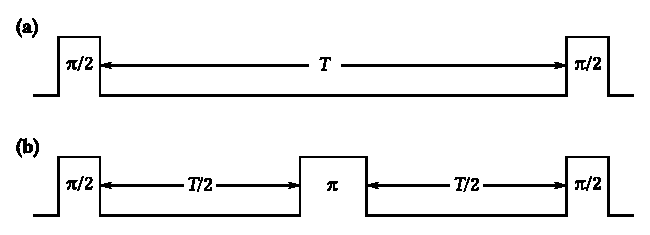
\includegraphics{figures_precreated/sequences.eps}}
    \caption[Timeline of Ramsey and spin echo experimental sequences]{
    Timeline of the experiment for \textbf{(a)} a regular Ramsey sequence, and \textbf{(b)} a Ramsey sequence with spin echo.}%endcaption
    \label{fig:bec-noise:visibility:sequences}
\end{figure}

The first protocol is a regular Ramsey sequence, depicted schematically in \figref{bec-noise:visibility:sequences},~(a): a $\pi/2$-pulse is applied by an electromagnetic coupler, creating a non-equilibrium superposition of components $\ket{1}$ and $\ket{2}$.
Mathematically, it means that coupling terms in~\eqnref{bec-noise:mean-field:cgpes-simplified} or in~\eqnref{bec-noise:wigner:single-particle-H} are enabled for a period of time equal to $t_{\mathrm{pulse}} = \theta / \Omega$, where $\theta = \pi/2$, with the Rabi frequency of the oscillator in this experiment being $\Omega = 350\un{Hz}$.
Since this pulse is short as compared to the total evolution time, it was simulated via an application of the rotation matrix~\eqnref{bec-noise:mean-field:rotation-matrix}.

During the further evolution of the system the components experience complex dynamics, separating and merging periodically~\cite{Mertes2007}.
This, in turn, leads to periodic dephasing and self-rephasing of the \abbrev{bec} components.
After some period of the free evolution, a second $\pi/2$-pulse is applied, transforming the phase difference between the two components in the superposition into a population difference which can be imaged.
Many such experiments are performed with different free evolution times, contributing one time-point each because the imaging effectively destroys the \abbrev{bec}.
A more detailed description of the experiment can be found in the paper by Egorov \textit{et~al}~\cite{Egorov2011}, and in his PhD thesis~\cite{Egorov2012}.
%acknowledgement
The experimental points used in this and the next section are also courtesy of M.~Egorov.

The simulations in this and the following sections used the plane wave basis (see \appref{bases} for details) and a $64\times8\times8$ spatial grid.
The integration was performed using a low-dissipation 4th-order Runge-Kutta algorithm (see \appref{numerical} for details).

The rephasing cycles can be represented by a common interferometric quantity~--- the fringe contrast, or visibility:
\begin{eqn}
\label{eqn:bec-noise:visibility:visibility}
    \mathcal{V}
    = \frac{2 \left| \int \langle \Psiop_1^\dagger \Psiop_2 \rangle \upd \xvec \right|}%
        {\int \langle \Psiop_1^\dagger \Psiop_1 + \Psiop_2^\dagger \Psiop_2 \rangle \upd \xvec},
\end{eqn}
where the denominator is just the total number of atoms in the system.
This quantity can be shown to be the envelope curve of the population fringes produced by the second $\pi/2$-pulse in the experiment.
In the mean-field model, the required correlations are calculated simply as
\begin{eqn}
    \tilde{n}
    & = \langle \Psiop_1^\dagger \Psiop_2 \rangle \approx \Psi_1^* \Psi_2, \\
    n_j
    & = \langle \Psiop_j^\dagger \Psiop_j \rangle \approx \Psi_j^* \Psi_j.
\end{eqn}
In the Wigner representation, we have to make the correlations symmetrically-ordered first, and then~\eqnref{wigner-bec:fpe-bec:moments} gives us
\begin{eqn}
    \tilde{n}
    & = \langle \Psiop_1^\dagger \Psiop_2 \rangle
    = \langle \symprod{ \Psiop_1^\dagger \Psiop_2 } \rangle
    \approx \Psi_1^* \Psi_2, \\
    n_j
    & = \langle \Psiop_j^\dagger \Psiop_j \rangle
    = \langle \symprod{ \Psiop_j^\dagger \Psiop_j }
        - \frac{\delta_{\restbasis_j}(\xvec, \xvec)}{2} \rangle
    \approx \pathavg{ \Psi_j^* \Psi_j } - \frac{M}{2V},
\end{eqn}
where we have used the fact that $\delta_{\restbasis_j}(\xvec, \xvec) \equiv M / V$ in the plane wave basis, where $M$ is the number of modes (for the grid we use $M = 64 \times 8 \times 8 = 4096$), and $V$ is the volume of the simulation area.

\begin{figure}
    \centerline{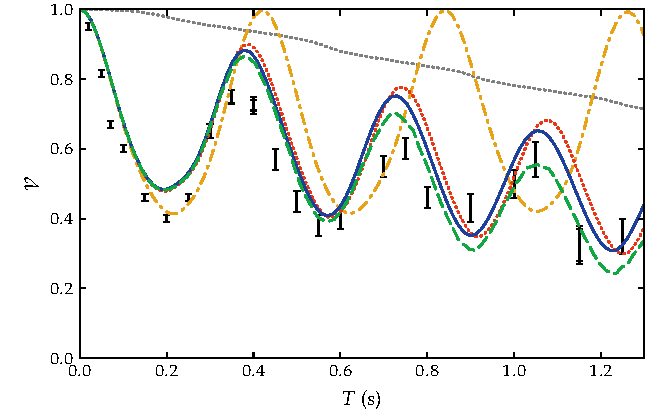
\includegraphics{figures_generated/bec_noise/ramsey_visibility_short.pdf}}

    \caption[Experimental and numerically simulated interferometric constrast in Ramsey sequence]{
    Comparison of experimental and numerically simulated interferometric contrast at the end of a regular Ramsey sequence with the evolution time $t$.
    Experimental results (black bars) are shown in comparison with the results given by the mean-field model (green dotted line), the truncated Wigner method (red dashed line), and the truncated Wigner with technical noises included (blue solid line).
    The mean-field results with losses turned off (yellow dash-dotted line) and the population-dependent visibility limit~\eqnref{bec-noise:visibility:limit} (grey dotted line) are included as a reference.}%endcaption

    \label{fig:bec-noise:visibility:ramsey-visibility}
\end{figure}

The visibility can serve as a good example of the differences introduced by taking into account losses, quantum effects, and technical noises in the simulation of the experiment.
The inclusion of these factors in the simulation of the Ramsey sequence is demonstrated in~\figref{bec-noise:visibility:ramsey-visibility}.
The experimental results and their uncertainties are shown as the black bars in the figure.

The simplest model~--- the mean-field \abbrev{cgpe}s~\eqnref{bec-noise:mean-field:cgpes-simplified} with losses turned off~--- gives results that are completely off base: the visibility is completely restored during rephasings (yellow dash-dotted lines in the figure).
This is to be expected as the theoretical limit of visibility
\begin{eqn}
\label{eqn:bec-noise:visibility:limit}
    \mathcal{V}_{\mathrm{max}}
    = \frac{2 \sqrt{N_1 N_2}}{N_1 + N_2},
\end{eqn}
where $N_1$ and $N_2$ are populations before the second $\pi/2$-pulse, equals to $1$ in this case, and there are no other limiting factors.

\begin{figure}
    \centerline{%
    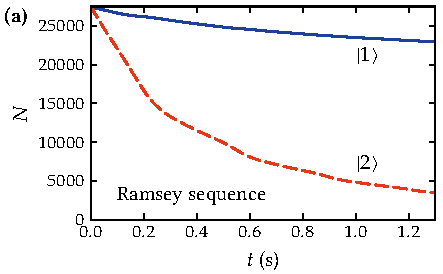
\includegraphics{figures_generated/bec_noise/ramsey_single_run_pop.pdf}%
    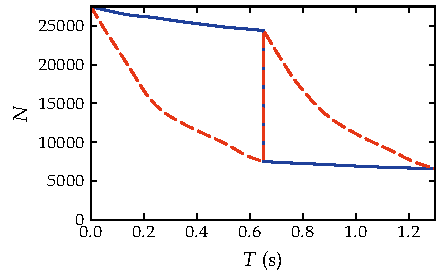
\includegraphics{figures_generated/bec_noise/echo_single_run_pop.pdf}}

    \caption[Component population in Ramsey and spin echo sequences]{
    Numerically simulated population of components $\ket{1}$ (blue solid lines) and $\ket{2}$ (red dashed lines) in \textbf{(a)} Ramsey and \textbf{(b)} spin echo sequences.}%endcaption

    \label{fig:bec-noise:visibility:population}
\end{figure}

But in the experiment in question the losses are present and are significantly asymmetrical as shown in~\figref{bec-noise:visibility:population},~(a).
With the populations typical for the experiment (tens of thousands of atoms or less), the two-body loss process in $\ket{2}$ is significantly stronger than the three-body one in $\ket{1}$.
This makes the theoretical limit~\eqnref{bec-noise:visibility:limit} decrease with time, as the dotted grey line in~\figref{bec-noise:visibility:ramsey-visibility} illustrates.
The resulting mean-field prediction with the inclusion of nonlinear losses (green dotted lines) is much closer to the experimental data.

The application of the \abbrev{sde}s~\eqnref{bec-noise:wigner:sde} obtained with the Wigner method (red dashed lines) has little effect on the short-time visibility (although it becomes more important at longer times as we will see later in~\figref{bec-noise:visibility:visibility-long}).
The Wigner results can be further adjusted to account for the noise introduced by the final measurement and non-ideal coupling (blue solid lines), which will be explained in detail in the next section.

The final agreement with the experiment is still not ideal, and the explanation of this difference is an open question.
Candidate factors include finite temperature effects and interaction with the surrounding cloud of non-condensed atoms.

\begin{figure}
    \centerline{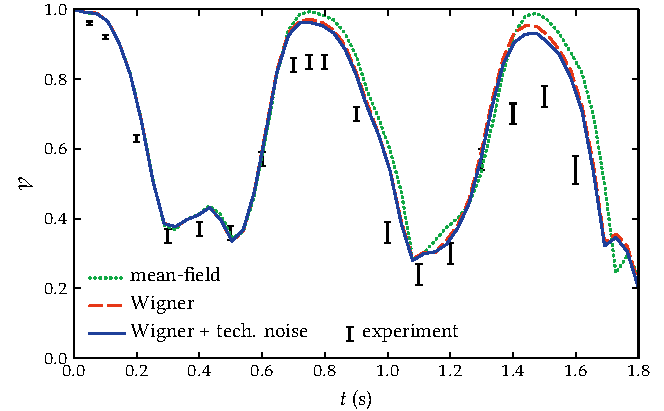
\includegraphics{figures_generated/bec_noise/echo_visibility_short.pdf}}

    \caption[Experimental and numerically simulated interferometric constrast in spin echo sequence]{
    Comparison of experimental and numerically simulated interferometric contrast at the end of a spin echo sequence with the evolution time $t$.
    Experimental results (black bars) show the final visibility value for a single spin echo sequence with the full evolution time $t$ as compared with the predictions from the mean-field model (green dotted line), the truncated Wigner method (red dashed line), and the truncated Wigner with technical noises included (blue solid line).}%endcaption

    \label{fig:bec-noise:visibility:echo-visibility}
\end{figure}

The asymmetricity introduced by the difference in loss rates can be compensated by periodically swapping the populations of the two components by a ``spin echo'' coupler pulse of the length $\pi$.
The simplest, yet already very effective, variant is to apply the $\pi$-pulse in the middle of the evolution as illustrated by~\figref{bec-noise:visibility:sequences},~(b).
With this additional pulse, by the end of a single experimental sequence the populations of two components become equal again as shown in~\figref{bec-noise:visibility:population},~(b), restoring the theoretical visibility limit~\eqnref{bec-noise:visibility:limit} back to $1$.

The mean-field model predicts the full recovery of the visibility even at long evolution times, which is inconsistent with the experiment as seen in~\figref{bec-noise:visibility:echo-visibility}.
On the other hand, the quasiprobability model qualitatively predicts the decay of visibility with time.
Same as in the case of the regular Ramsey sequence, the predictions of the simulation are improved by the inclusion of the technical noise.

\begin{figure}
    \centerline{%
    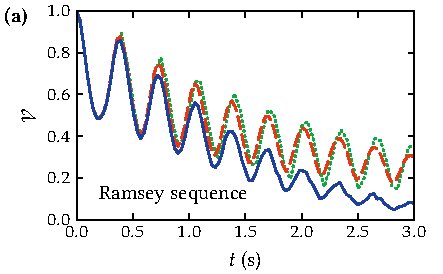
\includegraphics{figures_generated/bec_noise/ramsey_visibility_long.pdf}%
    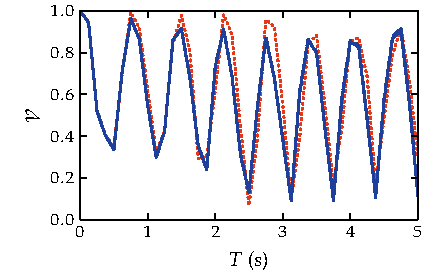
\includegraphics{figures_generated/bec_noise/echo_visibility_long.pdf}}

    \caption[Experimental and numerically simulated interferometric constrast in Ramsey and spin echo sequences for longer times]{
    Numerically simulated interferometric contrast for \textbf{(a)} a Ramsey sequence, and \textbf{(b)} a spin echo sequence at longer times.
    The results for the mean-field model (green dotted lines), the truncated Wigner method (red dashed lines) and the truncated Wigner with technical noises (blue solid lines) are plotted.}%endcaption

    \label{fig:bec-noise:visibility:visibility-long}
\end{figure}

The simulations can be performed for longer times as shown in~\figref{bec-noise:visibility:visibility-long}.
The difference between the mean-field and the truncated Wigner approach becomes clearer in~\figref{bec-noise:visibility:visibility-long},~(a), where the truncated Wigner predicts the significant decrease in the amplitude of the rephasing oscillations, caused by the quantum noise.
One must remember though that at such times the simulated atom densities become too low due to losses and violate the truncation validity criterion~\eqnref{wigner-bec:truncation:delta-condition}, thus making the predictions less reliable.
